\subsubsection{最大流}

\begin{itemize}

\item \textbf{判断一条边是否必定满流}

在残量网络中跑一遍 Tarjan,如果某条满流边的两端处于同一 SCC 中,则说明它不一定满流。(因为可以找出包含反向边的环,增广之后就不满流了。)

\end{itemize}

\subsubsection{最小割}

首先牢记最小割的定义:选权值和尽量小的一些边,使得删除这些边之后 $s$ 无法到达 $t$。

\paragraph{最小割输出一种方案}
在残量网络上从 $S$ 开始 floodfill,源点可达的记为 $S$ 集,不可达的记为 $T$ 集。如果一条边的起点在 $S$ 集而终点在 $T$ 集,就将其加入最小割中。

\paragraph{最小割的可行边与必须边}
\begin{itemize}
	\item 可行边: 满流,且残量网络上不存在 $u$ 到 $v$ 的路径,也就是 $u$ 和 $v$ 不在同一 SCC 中。(实际上也就是最大流必定满流的边。)

	\item 必须边:满流,且残量网络上 $S$ 可达 $u$,$v$ 可达 $T$。
\end{itemize}

\paragraph{字典序最小的最小割}
直接按字典序从小到大的顺序依次判断每条边能否在最小割中即可。

如果一条边是可行边,我们就需要把它删掉,同时进行退流,$u\to s$ 和 $t\to v$都 退掉等同于这条边容量的流量。

退流用 Dinic 实现即可。

% \subsubsection{费用流}


\subsubsection{上下界网络流}

\paragraph{无源汇上下界可行流}
新建源汇 $S', T'$,然后如图所示转化每一条边。

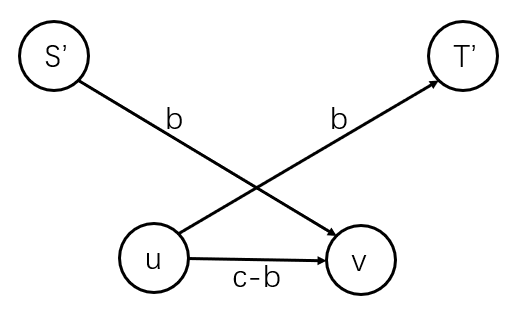
\includegraphics[scale = 0.5]{../src/graph/上下界网络流.png}

在新图跑一遍最大流之后检查一遍辅助边,如果有辅助边没满流则无解,否则把每条边的流量加上 $b$ 就是一组可行方案。

\paragraph{有源汇上下界最大流}
如果不需要判断是否有解的话,可以直接按照和上面一样的方法转化。因为附加边实际上算了两次流量,所以最终答案应该减掉所有下界之和。

(另外这里如果要压缩附加边的话,不能像无源汇的情况一样对每个点只开一个变量统计溢出的流量。正确的做法是进出流量各统计一下,每个点连两条附加边。)

如果需要判有解的话会出一点问题。这时候就需要转化成无源汇的情况,验证有解之后撤掉 $T$ 到 $S$ 的那条附加边,再从 $S$ 到 $T$ 跑一遍最大流。

\inputminted{cpp}{../src/graph/有源汇上下界最大流.cpp}

\paragraph{有源汇上下界最小流}
按照上面的方法转换后先跑一遍最大流,然后撤掉超级源汇和附加边,反过来跑一次最大流退流,最大流减去退掉的流量就是最小流。

\subsubsection{常见建图方法}

\begin{itemize}

\item \textbf{最大流/费用流}

流量不是很多的时候可以理解成很多条路径,并且每条边可以经过的次数有限。

\item \textbf{最小割}

常用的模型是 \textbf{最大权闭合子图}。当然它并不是万能的,因为限制条件可以带权值。

\begin{enumerate}

\item 如果某些点全部在 $S$ 集或者 $T$ 集,则获得一个正的收益

把这个条件建成一个点,向要求的点连 $+\infty$ 边,然后 $s$ 向它连 $+\infty$ 边。(如果是 $T$ 集就都反过来)

那么如果它在 $S$ 集,就一定满足它要求的点都在 $S$ 集,反之如果是 $T$ 集亦然。

\item 如果两个点不在同一集合中,则需要付出代价

建双向边,那显然如果它们不在同一集合中就需要割掉中间的边,付出对应的代价。

\item 二分图,如果相邻的两个点在同一集合则需要付出代价

染色后给一半的点反转源汇,就转换成上面的问题了。

\end{enumerate}

\end{itemize}

\subsubsection{例题}

\begin{itemize}

% \item 最大流



% \item 最小割

% \begin{enumerate}

% \item 切糕

% \end{enumerate}

\item 费用流

\begin{enumerate}

\item 序列上选总和尽量大的数,但连续 $k$ 个数中最多选 $p$ 个

费用流建图,先建一条 $n+1$ 个点的无限容量的链表示不选,然后每个 $i$ 向 $(i + k)$ 连边费用是第 $i$ 个位置的权值。答案是流量为 $p$ 的最大费用流,因为条件等价于选 $p$ 次并且每次选的所有数间隔都至少是 $k$。

\item 除此之外还要求连续 $k$ 个数中最少选 $q$ 个

任选一个位置把图前后切开,会发现通过截面的流量总和恰为 $p$。注意到如果走了最开始的链就代表不选,因此要限制至少有 $q$
的流量不走链,那么只需要把链的容量改成 $p - q$ 就行了。

\end{enumerate}

\end{itemize}
